\chapter{La unión PN}

Definimos como unión $pn$ a un semiconductor al cual se le aplica en una región un dopado tipo $p$ y en otra región un dopado tipo $n$, de tal modo que $N_A \gg N_D$ en $x<0$ y $N_D \gg N_A$ en $x>0$. El estudio y caracterización de la unión $pn$ es fundamental para entender la electrónica moderna. Existen 3 situaciones en las que podemos estudiar la unión pn, que son:

\begin{itemize}
    \item \textbf{Equlibrio termodinámico}, en el que no aplicamos una diferencia de potencial $V_A$ entre la  zona $p$ y zona $n$ externa.
    \item \textbf{Polarización directa} en el que aplicamos una diferencia de potencial $V_A>0$, es decir, polarizamos $p$ respecto $n$.
    \item \textbf{Polarización inversa} en el que aplicamos una diferencia de potencial $V_A<0$, es decir, polarizamos $n$ respecto $p$.
\end{itemize} 

\section{Equilibrio termodinámico}

\subsection{Introducción}

Entendemos por \textit{equilibrio termodinámico} a la situación en la que no hay corriente externa palicada, no hay iluminación y tampoco hay gradientes de la temperatura. Además consideramos las siguientes suposiciones:

\begin{itemize}
    \item Dispositivo unidimensional.
    \item Unión metalúrgica en $x_j=0$. 
    \item Contactos óhmicos perfectos.
\end{itemize} 
Debido a la aparición de esta diferencia de dopado aparece una región alrededor de $x=0$ en el que $n$ y $p$ se difunden, esto es, $n\neq N_D$ u $p\neq N_A$, tal que $n$ y $p$ dependen de $x$. A esta región la llamamos \textbf{zona de vaciamiento}, y en ella aparece un campo eléctrico no nulo en virtud de la ecuación de Maxwell-Poisson:

\begin{equation}
    \div \Encal = \frac{\rho}{K_S \varepsilon_0}
\end{equation}
siendo $\rho=-qn(x)+qp(x)$, y como $V(x)=-\int \Ecal \D x$, también aparece un potencial no constante (siempre en la zona de vaciamiento). Como sabemos, existe una relación entre $V$ y las energías $E_i,E_v$ y $E_c$. 

\begin{equation*}
    q \parciales{V}{x} = - \parciales{E_i}{x}
\end{equation*}
y como $E_F$ es contante en el equlibrio. Para conocer por completo la unión pn, lo que nosotros llamamos \textit{caracterizar la unión pn}, necesitamos conocer: 

\begin{itemize}
    \item Densidad de carga $\rho(x)$.
    \item Campo eléctrico $\Ecal(x)$.
    \item Potencial electrico $V(x)$.
    \item Anchuras de la región de vaciamiento $x_n$ y $x_p$.
    \item Esquema de bandas en todo el dispostivo. 
\end{itemize}
a partir de estos valores podemos concoer tanto corriente, como densidad de portadores... en todo el dispositivo. Definimos como \textbf{unión pn escalon} a aquella unión $pn$ en la que con regiones $p$ y $n$ dopados uniformemente, con un salto abrupto en $x=0$.. Es el caso más sencillo y más usado. El esquema de bandas es:

\begin{figure}[h!] \centering
    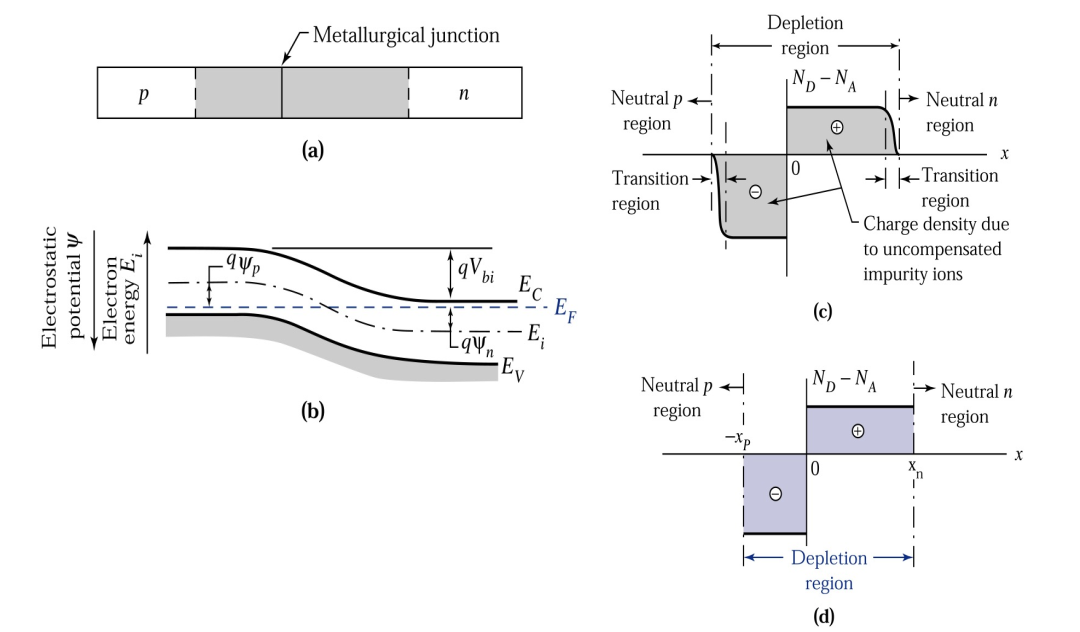
\includegraphics[width=0.9\linewidth]{Cuerpo/Ch_03/03_Temario_01.png}
\end{figure}
Cabe destacar que la caracterización de cualquier unión $pn$ (sea escalón, gradual...) es muy similar, presentando esquemas de bandas similares, solo cambiando la forma en la región de vaciamiento. Nosotros nos centraremos particularmente en la unión escalón, al ser la más sencilla. 

\subsection{Caracterización de la unión pn escalón}

Caracterizar la unión $pn$ es equivalente a conocer la densidad de carga, el campo eléctrico y el potencial a lo largo del dispositivo, a sí como la anchura de la región de vaciamiento. Muchos de estos valores están relacionados entre sí, y todos ellos dependen de el nivel de dopado $(N_D,N_A)$ del material ($E_g,n_i$) y de la temperatura ($T$). La mayor parte de estos los calcularemos a partir de aproximaciones. Lo que si podemos calcular sin hacer (casi) ninguna aproximación es $V_{bi}$, un parámetro que aparecerá recurrentemente. Hay dos maneras de calcular/definir $V_{bi}$, a saber, por energías y por corrientes. La definición por energías es la más sencilla, y por el que nosotros optamos. Básicamente nos dice que $\Vbi$ es la diferencia entre la región P y N del dispositivo para cualquiera de las bandas ($E_i,E_c,E_v$,). Así pues:

\begin{equation}
    \Vbi = -\frac{1}{q}(E_i|_P - E_i|_ N) = -\frac{kT}{q} \parentesis{\parentesis{-\ln\parentesis{p_p/n_i}}-\ln\parentesis{n_n/n_i}} = \frac{kT}{q} \ln \parentesis{\frac{N_AN_D}{n_i^2}}
\end{equation}
Asñ¡í pues, se define $\Vbi$ como:
\begin{equation}
    \Vbi= \frac{kT}{q} \ln \parentesis{\frac{N_AN_D}{n_i^2}} 
\end{equation}
Para calcular la anchura, campo eléctrico y potencial necesitamos sin embargo hacer la \textbf{aproximación a zona de vaciamiento}. Esta aproximación nos dice que la región comprendida entre $-x_p$ y $x_n$ (límites de la zona de vaciamiento) tanto $n$ como $p$ son despreciables frente $N_A$ y $N_D$, tal que:

\begin{itemize}
    \item En $-x_p\leq x \leq 0$ tenemos que $n_p,p_p\ll N_A^-$ y por tanto la densidad de carga $\rho(x)=-qN_A^-$.
    \item  En $0\leq x \leq x_n$ tenemos que $n_n,p_n\ll N_D^+$ y por tanto la densidad de carga $\rho(x)=qN_A^+$.
\end{itemize}
De esta forma la función de densidad de carga nos dice: 

\begin{equation}
    \rho(x) = \left\lbrace \begin{array}{ll}
        0 & \quad x < -x_p \\
        -qN_A & \quad   -x_p< x < 0  \\
        qN_D & \quad 0< x < x_n \\
        0 & \quad x_n < x    \\
    \end{array} \right.
\end{equation}
Y por tanto la corriente eléctrica tras integrar

\begin{equation}
    \Ecal (x) = \left\lbrace  \begin{array}{ll}
    0 & \quad x < -x_p \\
    \frac{-q N_A}{K_S\epsilon_0} (x+x_p) & \quad   -x_p< x < 0  \\
    \frac{q N_D}{K_S\epsilon_0} (x-x_n)& \quad 0< x < x_n \\
    0 & \quad x_n < x    \\ 
    \end{array}  \right.
\end{equation}
Y el potencial eléctrico tras inegrar el campo eléctrico: 
\begin{equation}
    V (x) = \left\lbrace  \begin{array}{ll}
    0 & \quad x < -x_p \\
    \frac{q N_A}{2K_S\epsilon_0} (x+x_p)^2 & \quad   -x_p< x < 0  \\
    \frac{q N_D}{2K_S\epsilon_0} (x-x_n)^2 + \Vbi & \quad 0< x < x_n \\
    \Vbi & \quad x_n < x    \\
    \end{array}  \right.
\end{equation}
donde $K_S$ es  el \textbf{coeficiente de permitividad relativa}. A partir de la exigencia de continuidad de $V(x)$ y de su derivada $\Ecal(x)$ a lo largo del dispositivo podemos hallar $x_n$ y $x_p$, ya que: 

\begin{equation}
    \Ecal(0^+) = \Ecal(0^-) \ \Longrightarrow N_A x_p = N_D x_n
\end{equation}
\begin{equation}
    V(0^+) = V(0^-) \ \Longrightarrow N_A x_p^2 = -N_D x_n^2 + \Vbi
\end{equation}
de lo que se puede deducir que: 

\begin{equation}
    x_n = \ccorchetes{\frac{2K_S\epsilon_0 \Vbi}{q} \frac{N_A}{N_D(N_A+N_D)}}^{1/2} \qquad 
    x_p = \ccorchetes{\frac{2K_S\epsilon_0 \Vbi}{q} \frac{N_D}{N_A(N_A+N_D)}}^{1/2}
\end{equation}

\subsection{Caracterización de la unión pn gradual}

%%%%%%%%%%%%%%%%%%%%%%%%%%%%%%%%%%%%%%%%%%%%%%%%%%%%%%%%%%%%%%%%%%%%%%%
%%%%%%%%%%%%%%%%%%%%%%%%%%%%%%%%%%%%%%%%%%%%%%%%%%%%%%%%%%%%%%%%%%%%%%%
%%%%%%%%%%%%%%%%%%%%%%%%%%%%%%%%%%%%%%%%%%%%%%%%%%%%%%%%%%%%%%%%%%%%%%%
%%%%%%%%%%%%%%%%% UNION PN BAJO POLARIZACIONES %%%%%%%%%%%%%%%%%%%%%%%%
%%%%%%%%%%%%%%%%%%%%%%%%%%%%%%%%%%%%%%%%%%%%%%%%%%%%%%%%%%%%%%%%%%%%%%%
%%%%%%%%%%%%%%%%%%%%%%%%%%%%%%%%%%%%%%%%%%%%%%%%%%%%%%%%%%%%%%%%%%%%%%%
%%%%%%%%%%%%%%%%%%%%%%%%%%%%%%%%%%%%%%%%%%%%%%%%%%%%%%%%%%%%%%%%%%%%%%%

\section{Union pn bajo polarizaciones} \label{Sec:03-02}

Decimos que una unión PN o diodo está polarizado cuando estamos aplicando una diferencia de potencial entre la zona n y la zona p externamente, tal como se puede ver en la siguiente imagen: 

\begin{figure}[h!] \centering
    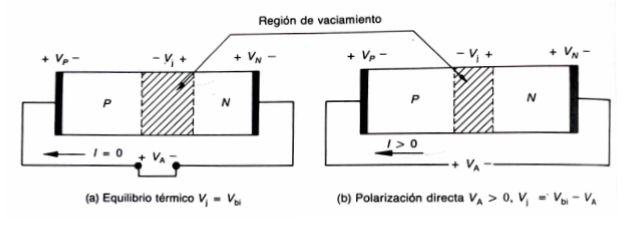
\includegraphics[width=0.7\linewidth]{Cuerpo/Ch_03/03_Temario_05.png}
\end{figure}
De esta manera definimos:

\begin{itemize}
    \item $V_j$: caída de tensión entre $n$ y $p$.
    \item $V_P$: caída de tensión entre $p$ y el metal.
    \item $V_N$: caída de tensión entre $n$ y el metal.
    \item $V_A$: caída de tensión externa.
\end{itemize}
Para obtener la relación entre $V_j$, qué es al final el valor que hay entre las bandas en $N$ y $P$, así como la altura del potencial $V(x)$ entre los extremos de la región de vaciamiento, es necesiario observar muy bien la imagen anterior y ver como se colocan los + y los - en la imagen. Usando las mallas tendríamos que: 

\begin{equation}
    V_j = \Vbi - V_N - V_A - V_P
\end{equation}
Como en general, las uniones metalúrgicas son perfectas tendremos que $V_N=V_P=0$, tal que así: 


\begin{equation}
    V_j = \Vbi - V_A
\end{equation}
Entonces todas las ecuacioens qeu anteriormente usamos con $\Vbi$ en el equlibrio tendremos que sustituirlas por $V_j$. Lo primero que podmeos notar es que en función de $V_A$ las región de vaciamiento se hace mas grande o disminuye: 


\begin{equation}
    x_n = \ccorchetes{\frac{2K_S\epsilon_0 }{q} (\Vbi - V_A) \frac{N_A}{N_D(N_A+N_D)}} \qquad 
    x_p = \ccorchetes{\frac{2K_S\epsilon_0 }{q} (\Vbi - V_A) \frac{N_D}{N_A(N_A+N_D)}}
\end{equation}
por lo que, aún no afectando al campo eléctrico o la densidad de carga de manera directa, solo por el hecho de cambiar la región de vaciamiento ya ha cambiado la forma funcional de estas ecuaciones (por ejemplo $\Ecal_{\max}$), y sobre todo la distancia entre bandas:

\begin{equation}
    E_i|_P-E_i|_N=V_j \quad  E_c|_P-E_c|_N=V_j \quad  E_v|_P-E_v|_N=V_j
\end{equation}

Diferenciamos dos polarizaciones: 

\begin{itemize}
    \item La \textbf{polarización directa} $V_A>0$. En la polarización directa tamaño de la región de vaciamiento se reduce, lo que reduce el campo eléctrico máximo, y lo que es más importante, disminuye la distancia entre bandas $E_i|_N$ e $E_i|_P$, lo que hace más fácil que los electrones/huecos se muevan en la región de vaciamiento (ya que tienen menos potencial que superar) haciendo que aparezca una corriente eléctrica no nula entre ambos puntos. 
    \item La \textbf{polarización inversa} $V_A<0$. En la polarización inversa tamaño de la región de vaciamiento aumenta, lo que aumenta el campo eléctrico máximo, y lo que es más importante, aumenta distancia entre bandas $E_i|_N$ e $E_i|_P$.
\end{itemize}





%%%%%%%%%%%%%%%%%%%%%%%%%%%%%%%%%%%%%%%%%%%%%%%%%%%%%%%%%%%%%%%%%%%%%%%
%%%%%%%%%%%%%%%%%%%%%%%%%%%%%%%%%%%%%%%%%%%%%%%%%%%%%%%%%%%%%%%%%%%%%%%
%%%%%%%%%%%%%%%%%%%%%%%%%%%%%%%%%%%%%%%%%%%%%%%%%%%%%%%%%%%%%%%%%%%%%%%
%%%%%%%%%%%%%% CARACTERISTICAS IV DE LA UNION PN %%%%%%%%%%%%%%%%%%%%%%
%%%%%%%%%%%%%%%%%%%%%%%%%%%%%%%%%%%%%%%%%%%%%%%%%%%%%%%%%%%%%%%%%%%%%%%
%%%%%%%%%%%%%%%%%%%%%%%%%%%%%%%%%%%%%%%%%%%%%%%%%%%%%%%%%%%%%%%%%%%%%%%
%%%%%%%%%%%%%%%%%%%%%%%%%%%%%%%%%%%%%%%%%%%%%%%%%%%%%%%%%%%%%%%%%%%%%%%

\section{Características IV de la union pn}

En una situación de equilibrio la densidad de electrones $n$ en la zona $n$ de la unión será mucho mayor que en la zona $p$. Esta diferencia de densidades provocará la aparición de una corriente de difusión de la región $n$ a la región $p$. Sin emargo, la existencia de una diferencia de potencial entre la zona $n$ y la zona $p$ genera un campo eléctrico contrario a la corriente de difusión. En el equilibrio estas dos corrientes estań compensadas, de tal modo que:

\begin{equation}
    \text{Equlibrio:} \ \Jn_n = \Jn_p = 0
\end{equation}
Sin embargo cuando aplicamos un voltaje a la union pn, el equilibrio entre la densidad de corriente debida al campo eléctrico y la corriente de difusión desaparecerá, de tal modo que aparecerá una corriente eléctrica no nula a través del dispositivo. 

Bajo una corriente directa $V_A>0$, el potencial se reducirá (tal y como hemos visto en la sección anterior), lo que conlleva una disminución del campo eléctrico \cref{Fig:03_01}.

\begin{figure}[h!]
\centering
\begin{subfigure}{0.47\textwidth}
    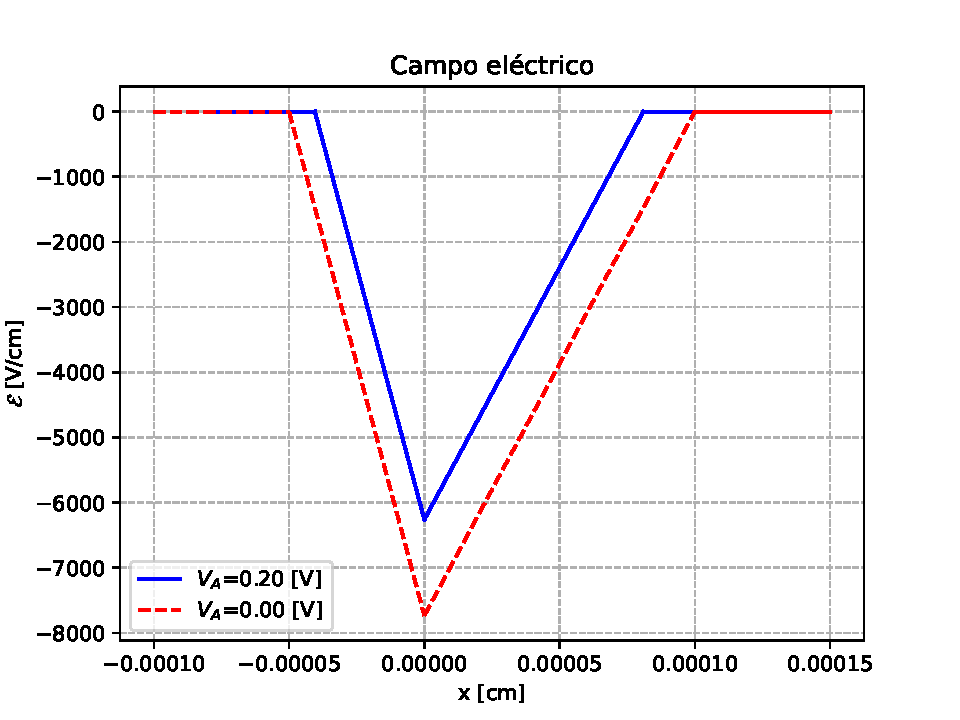
\includegraphics[width=\textwidth]{Cuerpo/Ch_03/03_04_E.pdf}
\end{subfigure}
\begin{subfigure}{0.47\textwidth}
    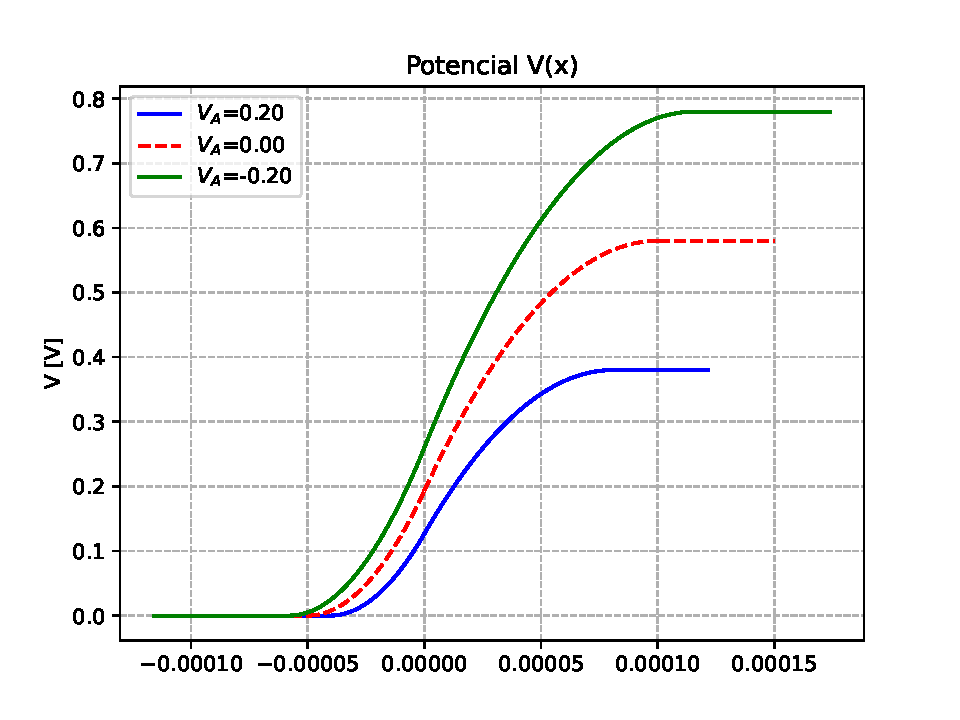
\includegraphics[width=\textwidth]{Cuerpo/Ch_03/03_05_V.pdf}
\end{subfigure}
\caption{Campo eléctrico y potencial para diferentes valores de $V_A$.}
\label{Fig:03_01}
\end{figure}
reduciendo la corriente eléctrica de arrastre. Además de esto, que el potencial eléctrico sea más pequeño hace que los electrones/huecos tengan que superar una barrera de potencial más pequeña para pasar al otro lado por difusión, facilitando así que los electrones/huecos en la región masiva $N$/$P$ o región $n/p$ pasen al a región masiva $P/N$. Consecuentemente, los portadores minoritarios pueden comenzar a inyectarse, esto es, los electrones comenzarán a inyectarse en la región masiva $P$ y los huecos en la región masiva $N$. 

Por otro lado, cuando $V_A<0$, el fenómeno es justamente el contrario, la barrera de potencial aumenta de tal manera que menos electrones se inyectan en la región $P$ y menos huecos en la región $N$. Esto provoca una disminución en la difusión de los portadores, y por tanto se reduce la posible corriente por difusión que pudiera haber. La corriente que aparece bajo polarización inversa se debe a la corriente de arrastre (corriente debida a $\Ecal \neq 0$) producida por el efecto del campo eléctrico sobre los portadores minoritarios. Un número minoritario de electrones/huecos en la región $p/n$ serán arrastrados a la región $n/p$, la corriente de arrastre depende principalmente de del número de portadores minoritarios, que viajarán a la velocidad de saturación. 

En cualquier caso, en la región de vaciamiento existen ambos fenómenos simultáneamente, lo que complica bastante su cálculo. Por tanto el calculo de las corrientes de difusión tienen que hacer fuera de la región de vaciamiento. En esta sección trataremos de calcular las relaciones intensidad-voltaje (IV), a través de diferentes aproximaciones.

\subsection{Aproximación del diodo ideal}

La \textbf{ecuación del diodo ideal} o \textbf{aproximación del diodo ideal} nos permite calcular analíticamente (y de manera sencilla) las relaciones de corriente $J$ (tanto de difusión como de arrastre) en función de la posición del diodo y el valor del potencial $V_A$. Las aproximaciones son:

\begin{itemize}
    \item No hay fuentes externas de generación de portadores (iluminación).
    \item Son aplicables las aproximaciones de vaciamiento anteriores y de unión escalón.
    \item Solución en estado estacionario (las densidades $n$ y $p$ son constantes a lo largo de la unión).
    \item No existe recombinación ni generación de portadores en la región de vaciamiento. 
    \item Se mantiene bajo nivel de inyección en las regiones masivas. El campo eléctrico es cero en las regiones masivas: toda la tensión cae en la zona de vaciamiento.
    \item La resistiviadad de las regiones masivas o casi neutras es lo suficientemente pequeña como para que el paso de corriente no provoque caídas de tensión. Toda la tensión cae en las zona de vaciamiento. 
    \item Las regiones masivas están dopadas uniformemente.
    \item La densidad de los portadores móviles en la zona de vaciamiento es aproximadamente la que tendŕiamos en equilibrio, pero con una barrera de potencial desplazada con la tensión aplicada. Los cuasi-niveles de Fermi son constantes en la zona de transición. 
\end{itemize}

\subsection{Diodo ideal: corrientes en las zonas masivas}

Tal y como hemos visto, estas condiciones de los portadores minoritarios sobre la zona fuera de la región de vaciamiento se parecen mucho a las condición 1 de \cref{Subsec:02-04-02}: \textit{situación estacionaria y sin iluminación}. Así pues, siempre podemos aplicar las mismas ecuaciones sobre $\Delta p_n$ y $\Delta n_p$:

\begin{equation}
    \text{Zona P:} \ D_N \derivadas{^2 \Delta n_p}{ x^2} - \frac{\Delta n_p}{\tau_n} = 0 
\end{equation}
\begin{equation}
    \text{Zona N:} \ D_P \derivadas{^2 \Delta p_n}{ x^2} - \frac{\Delta p_n}{\tau_p} = 0
\end{equation}
La solución es, en la resgiones masivas

\begin{equation}
    \text{Zona P:} \
    \Delta n_p = A e^{-x/L_N} + B e^{x/L_N} \qquad 
    \text{Zona N:}  \
    \Delta p_n = A' e^{-x/L_P} + B' e^{x/L_P}
\end{equation}
tal que $L_N=\sqrt{D_N\tau_n}$ y $L_P=\sqrt{D_P\tau_p}$. En la \cref{Fig:03_02} aparecen las dependencias exponenciales que vemos tanto en polarización directa como en polarización inversa, tanto en las regiones mastivas como en las zona de vaciamiento.
\begin{figure}[h!] \centering
    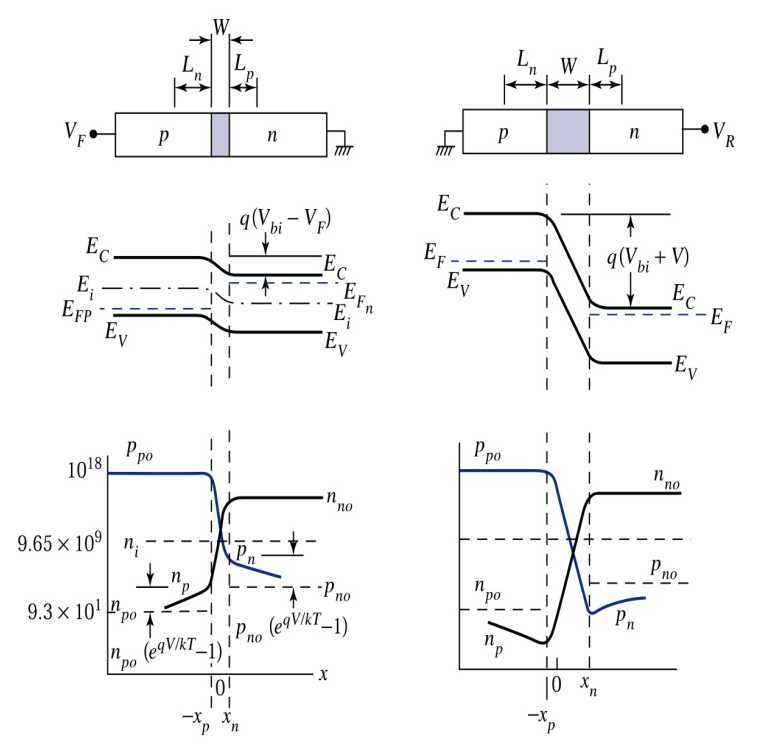
\includegraphics[width=0.6\linewidth]{Cuerpo/Ch_03/03_Temario_02.png}
    \caption{Portadores minoritarios a lo largo del dispositivo pn.}
    \label{Fig:03_02}
\end{figure}
Ahora tendremos que aplicar las condiciones de cotorno. La primera condición de contorno es que $n_p(-\infty)=0$ y que $p_n(\infty)=0$. Esto hace que $A=0$ y que $B'=0$, tal que:

\begin{equation}
    \text{Zona P:} \
    \Delta n_p = B e^{x/L_N} \qquad 
    \text{Zona N:}  \
    \Delta p_n = A' e^{-x/L_P} 
\end{equation}
La segunda condición de contorno tiene que darse justo cuando empieza la región de vaciamiento, esto es, en $x_n$ (para $p_n$) y en $x_p$ (para $n_p$). Para obtener la condición empezamos por:
\begin{equation}
    \Vbi = \frac{kT}{q} \ln  \parentesis{\frac{N_AN_D}{n_i^2}} \approx  \frac{kT}{q} \ln  \parentesis{\frac{p_{p0}n_{n0}}{n_i^2}}
\end{equation}
siendo $p_{p0}$ la cantidad de portadores tipo hueco que hay en la región masiva $P$ en el equlibrio y $n_{n0}$ la cantidad de portadores tipo electrón que hay en la región masiva $N$ en el equlibrio. Como sabemos $n_{p0}=n_i^2/p_{p0}$ y $p_{n0}=n_i^2/n_{n0}$, por lo que:

\begin{equation}
    n_{p0} = n_{n0} e^{-q\Vbi /kT}  \tquad
    p_{n0} = p_{p0} e^{-q\Vbi /kT}
\end{equation}
Así que cuando aplciamos un potencial externo tal que $\Vbi\rightarrow \Vbi- V_A$ (recordemos que una de las hipótesis es que toda la tensión aplicada $V_A$ cae en la zona de vaciamiento) llegamos a que:

\begin{equation}
    n_{p} |_{x_p}= n_{n0} e^{-q(\Vbi-V_A) /kT}  \tquad
    p_{n} |_{x_n}= p_{p0} e^{-q(\Vbi-V_A)/kT}
\end{equation}
tal que 

\begin{equation}
    \Delta n_p |_{x_p} = n_{p}-n_{p0} = n_{p0} \parentesis{ e^{qV_A/kT}  -1} \qquad 
    \Delta p_n |_{x_n} = p_{n}-p_{n0} = p_{n0} \parentesis{ e^{qV_A/kT}  -1}
\end{equation}
de lo que se deduce que \textit{las difernecias de portadores minoritarios respecto el equilibrio en las zonas masivas}

\begin{equation}
    \Delta n = n_{p0} \parentesis{e^{qV_A/kT}-1} e^{(x+x_p)/L_N} \tquad 
    \Delta p = p_{n0} \parentesis{e^{qV_A/kT}-1} e^{(x-x_n)/L_P}
\end{equation}
y consecuentemente \textbf{los portadores minoritarios en las zonas masivas}

\begin{equation}
     n_p = n_{p0} + n_{p0} \parentesis{e^{qV_A/kT}-1} e^{(x+x_p)/L_N} \tquad 
     p_n = p_{n0} + p_{n0} \parentesis{e^{qV_A/kT}-1} e^{(x-x_n)/L_P}
\end{equation}
En las zonas masivas solo puede haber corriente producida por la difusión (no hay campo electrico), tal que:

\begin{equation} 
    \text{Zona P:} \ J_N \simeq qD_N \derivadas{\Delta n_p}{x} \qquad \text{Zona N:} \ J_P \simeq -qD_P \derivadas{\Delta p_n}{x}
\end{equation}
por lo que \textbf{las corrientes en las zonas masivas}

\begin{equation}
    J_N (x) = \frac{qD_N}{L_N} n_{p0} \parentesis{e^{qV_A/kT}-1} e^{(x+x_p)/L_N} \qquad -\infty \leq x \leq -x_p \end{equation} \begin{equation} J_P (x) = \frac{qD_P}{L_P} p_{n0} \parentesis{e^{qV_A/kT}-1} e^{-(x-x_n)/L_P} \qquad x_n \leq x \leq \infty
\end{equation}

\subsection{Diodo ideal: corrientes en la zona de vaciamiento}

Por definición la corriente total tanto en la zona de vaciamiento como en la zonas masivas es constante \cref{Fig:03_03} e igual en todo punto del diodo (ya que la presencia de un punto con mas o menos corriente que otro provocaría la acumulación de carga en un sitio, lo que sería contrario a las hipótesis de solución estacionaria). Esto mismo lo aplicaremos en el apartado siguiente. Consecuentemente la corriente debida a las cargas hueco $J_P$ en la zona de vaciamiento debe ser igual a $J_P|_{\text{difusion}} (x_n)$, y la corriente debida a las cargas electrón $J_N$ en la zona de vaciamiento debe ser igual a $J_N|_{\text{difusion}} (x_p)$:

\begin{equation}
    J_P |_{\text{vaciamiento}} = J_P|_{\text{difusion}} (x_n) = - q D_N  \ \eval{\parciales{p_n}{x}}_{x=x_n} \end{equation}
\begin{equation}     
    J_N |_{\text{vaciamiento}} = J_N|_{\text{difusion}} (-x_p) =  q D_P  \ \eval{\parciales{n_p}{x}}_{x=x_p}
\end{equation}

\subsection{Ecuación del diodo ideal}

Como ya hemos dicho, por definición la corriente total tanto en la zona de vaciamientoc \cref{Fig:03_03} como en la zonas masivas es constante e igual en todo punto del  diodo:
\begin{equation}
    J =  J_N (-x_p) + J_P (x_n) = q \parentesis{\frac{D_N}{L_N} n_{p0} + \frac{D_P}{L_P} p_{n0}} \parentesis{e^{qV_A/kT}-1}
\end{equation}
Y si multiplicamos por el área transversal $A$ obtenemos:

\begin{equation}
    I = I_0 \parentesis{e^{qV_A/kT}-1} \qquad  I_0 =  A q \parentesis{\frac{D_N}{L_N} n_{p0} + \frac{D_P}{L_P} p_{n0}}
\end{equation}
Por tanto la intensidad dende del dopado, el coeficiente de difusión, el tipo de material y el voltaje de polarización $V_A$. Esta última dependencia se encuentra en \cref{Fig:03_03} (derecha). Otra forma de escribir $I_0$ es:

\begin{equation}
    I_0 = qA \parentesis{\frac{D_N}{L_N} \frac{n_i^2}{N_A} + \frac{D_P}{L_P} \frac{n_i^2}{N_D}}
\end{equation}
Esto nos lleva a una conclusión interesante: el lado menos dopado de la unión PN produce más cantidad de portadores minoritarios, lo que implica una mayor componente de corriente. Hay dos casos especiales, la unión P$^+$N $N_A \gg N_D $ y la unión N$^+$P $N_D\gg N_A$. 

\begin{figure}[h!]
    \centering
    \begin{subfigure}{0.47\textwidth}
        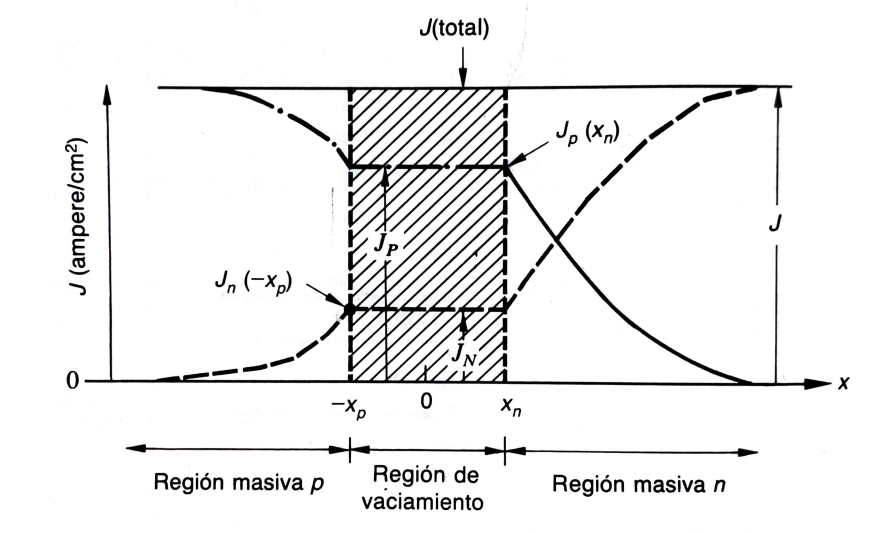
\includegraphics[width=\textwidth]{Cuerpo/Ch_03/03_Temario_03.png}
    \end{subfigure}
    \begin{subfigure}{0.47\textwidth}
        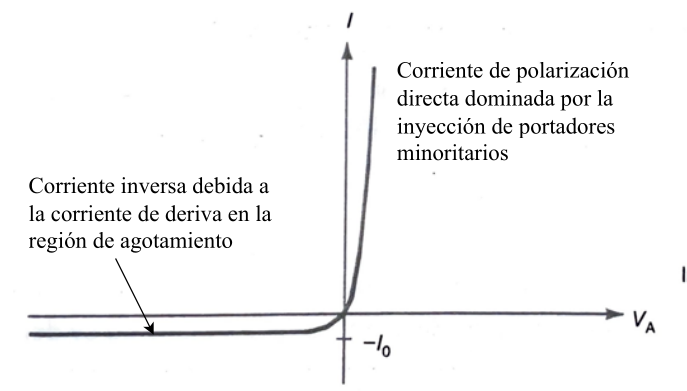
\includegraphics[width=\textwidth]{Cuerpo/Ch_03/03_Temario_04.png}
    \end{subfigure}
    \label{Fig:03_03}
    \caption{Corriente total y valor de la intensidad frente a $V_A$.}
\end{figure}

\subsection{Diodo estrecho}

Decimos que un diodo ideal es un \textbf{diodo estrecho} cuando uno de los lados del diodo $x_{1p}$ o $x_{1n}$ es proporcional a $L_N$ o $L_P$  respectivamente. Cuando es así no podemos aplicar la solución $\Delta n (-\infty) = 0$ o $\Delta p (\infty) = 0$, si no que tenemos que aplicar la siguiente condición:

\begin{equation}
    \Delta n  (x_{1p}) = 0 \qquad \Delta p (x_{1n}) = 0
\end{equation}
Consecuentemente tenemos que los valores de las constantes $A$, $B$, $A'$ y $B'$ cambian. La solución final acaba siendo:

\begin{equation}
    \Delta n_p (x) = n_{p0} \parentesis{e^{qV_A/kT}-1} \frac{\sinh \parentesis{\frac{x+x_{1p}}{L_N}}}{\sinh \parentesis{\frac{-x_{p}+x_{1p}}{L_N}}}
\end{equation}
\begin{equation}
    \Delta p_n (x) = p_{n0} \parentesis{e^{qV_A/kT}-1} \frac{\sinh \parentesis{\frac{x-x_{1n}}{L_P}}}{\sinh \parentesis{\frac{x_{n}-x_{1n}}{L_P}}}
\end{equation}
De tal modo que las corrientes ahora son:

\begin{equation}
    I_n (x) = qA \frac{D_N}{L_N} n_{p0} \frac{\cosh \parentesis{\frac{x_{1p}-x}{L_N}}}{\sinh \parentesis{\frac{x_{1p}-x_p}{L_N}}} \parentesis{e^{qV_A/kT}-1}
\end{equation}
\begin{equation}
    I_p (x) = qA \frac{D_P}{L_P} p_{n0}  \frac{\cosh\parentesis{\frac{x_{1n}-x}{L_P}}}{\sinh \parentesis{\frac{x_{1n}-x_n}{L_P}}}  \parentesis{e^{qV_A/kT}-1}
\end{equation}
Así pues, tenemos que 

\begin{equation}
    I = qA\ccorchetes{\frac{D_Pp_{n0}}{L_P} \coth \parentesis{\frac{x_{1n}-x_n}{L_P}}+\frac{D_N n_{p0}}{L_N} \coth \parentesis{\frac{x_{1p}-x_p}{L_N}}}
\end{equation}


%%%%%%%%%%%%%%%%%%%%%%%%%%%%%%%%%%%%%%%%%%%%%%%%%%%%%%%%%%%%%%%%%%%%%%%
%%%%%%%%%%%%%%%%%%%%%%%%%%%%%%%%%%%%%%%%%%%%%%%%%%%%%%%%%%%%%%%%%%%%%%%
%%%%%%%%%%%%%%%%%%%%%%%%%%%%%%%%%%%%%%%%%%%%%%%%%%%%%%%%%%%%%%%%%%%%%%%
%%%%%%%%%%%%%%% DESVIACIONES RESPECTO UNION IDEAL %%%%%%%%%%%%%%%%%%%%%
%%%%%%%%%%%%%%%%%%%%%%%%%%%%%%%%%%%%%%%%%%%%%%%%%%%%%%%%%%%%%%%%%%%%%%%
%%%%%%%%%%%%%%%%%%%%%%%%%%%%%%%%%%%%%%%%%%%%%%%%%%%%%%%%%%%%%%%%%%%%%%%
%%%%%%%%%%%%%%%%%%%%%%%%%%%%%%%%%%%%%%%%%%%%%%%%%%%%%%%%%%%%%%%%%%%%%%%


\section{Desviaciones respecto la unión ideal}

Las desviacionesen polarizaciones en polarización inversa y directa más generales: 

\begin{itemize}
    \item Desviaciones en polarización inversa:
    \begin{itemize}
        \item Ruptura de avalancha.
        \item Ruptura Zéner.
        \item Generación en la región de vaciamiento.
        \item Perforación.
    \end{itemize}
    \item Desviaciones en polarización directa: 
    \begin{itemize}
        \item Recombinación en la región de vaciamiento.
        \item Inyección de alto nivel.
        \item Efectos en al región masiva.
    \end{itemize}
\end{itemize}

\subsection{Desviaciones en polarización inversa}

Definimos como \textbf{voltaje de ruptura} $V_{BR}$ es el voltaje para el cual la corriente tiende a $-\infty$. El diodo se comporta como una fuente de voltaje fijo (diodo regulador) para un amplio intervalo de corriente (limitado por la potencia máxima que podría disipar). 

\begin{itemize}
    \item Avalancha.
    \item Zéner.
\end{itemize}
Luego además tenemos otros fenómenos, como las correnciones a $I_0$ debido a la generación/recombinación, o la perforación, que se produce cuando la región de vaciamiento ocupa todo el diodo. En la siguiente imagen podemos ver como se modifica $I$ en función de $V$ para el diodo real en polarización inversa: 


\begin{figure}[h!] \centering
    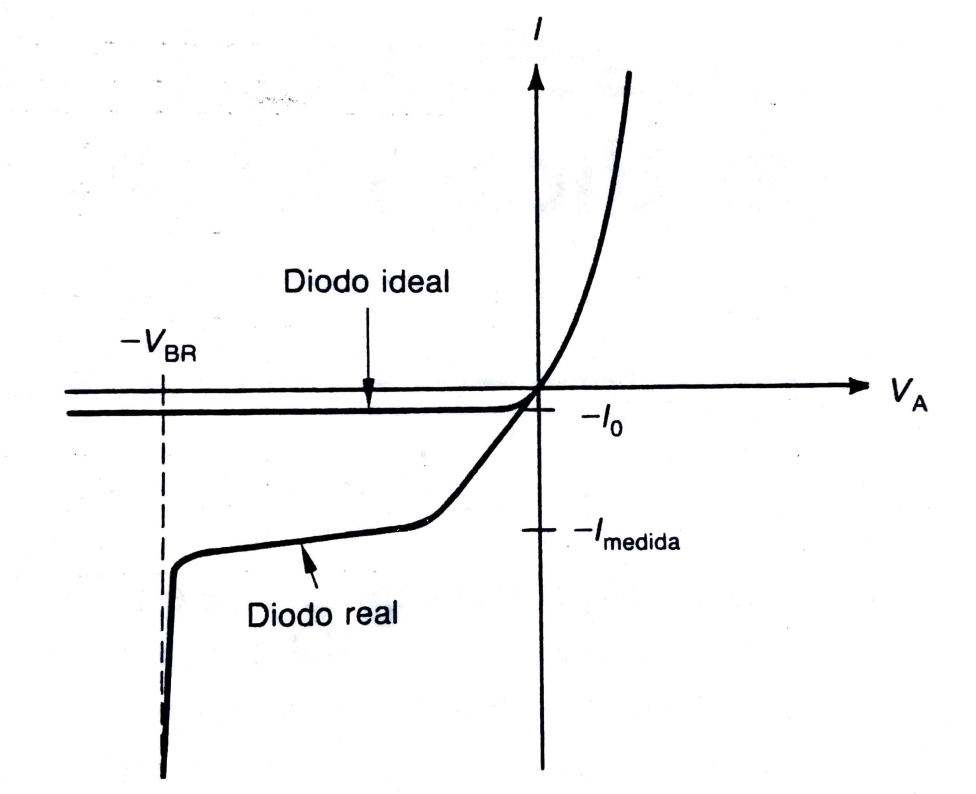
\includegraphics[width=0.5\linewidth]{Cuerpo/Ch_03/03_Temario_10.png}
    \caption{Corriente I respecto V en polarización inversa.}
\end{figure}

\subsubsection{Ruptura por avalancha}

La \textbf{ruptura por avalancha o ionización por impacto} para un valor crítico del campo eléctrico, os portadores se aceleran a un valor de energía suficientemente grande para que, cuando haya colisiones con un átomo de la estructura cristalina, puedan liberar un par electrón-hueco. Estos portadores liberados son acelerados por el campo eléctrico, lo que produce nuevas colisioens y nuevos portadores, generando una avalancha. Tiene dependencias con el dopado y la tempratura: 

\begin{figure}[h!] \centering
    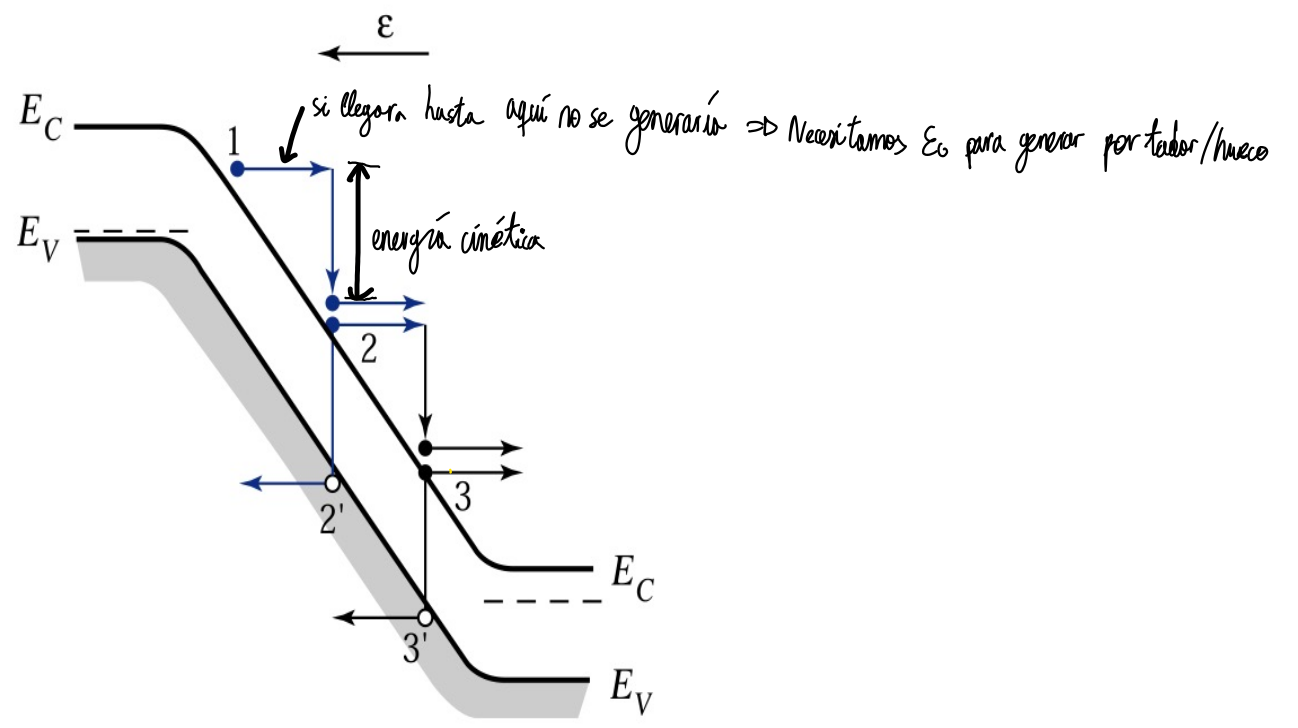
\includegraphics[width=0.7\linewidth]{Cuerpo/Ch_03/03_Temario_06.png}
    \caption{Ruptura por Avalancha.}
\end{figure}
La pregunta interesante aquí es saber cual es el valor del campo eléctrico que genera esta ruptura por avalancha. Como sabemos el campo máximo es $\Ecal(0)$, tal que:

\begin{equation}
    \Ecal_{\min} = - \frac{qN_D}{K_S\epsilon_0} x_n 
 \end{equation}
de tal manera que para un $V_A$ cualquiera podemos obtener un campo eléctrico mínimo. Si el \textbf{potencial de ruptura} es $V_{\text{BR}}$, existe campo eléctrico asociado a este potencial de ruptura $\Ecal_{\text{CR}}$  que se le llama \textbf{campo crítico} y \textit{es una constante física para cada semiconductor}. La relación entre ambos: 

\begin{equation}
  \Ecal_{\text{CR}}^2  = - \frac{2q}{K_S\epsilon_0} \parentesis{\Vbi-V_{\text{BR}}} \frac{N_AN_D}{N_A+N_D}
\end{equation}
despejando el potencial de ruptura:

\begin{equation}
    V_{\text{BR}}^2  = -\Vbi - \frac{K_S\epsilon_0}{2q} \frac{N_A+N_D}{N_AN_D} \Ecal_{\text{CR}}^2
  \end{equation}
Como podemos ver, si aumentamos el dopado disminuye el potencial de ruptura. 

\subsubsection{Ruptura por efecto túnel}

La rutpura zéner o ruptura pro efecto túnel se produce en las uniones PN fueremtente dopadas a ambos lados de la unión, ya que cuanto más dopado más pequeño es la anchura de la región de vaciamiento. Las condiciones para que se de: 

\begin{itemize}
    \item Una barrera de potencial delgada, véase por dopado alto. 
    \item Gran cantidad de electrones disponibles para este efecto túnel a un lado de la barrera y una gran cantidad de estados vacíos al mismo nivel de energía al otro lado. 
\end{itemize}
Como podemos ver en la imagen siguiente, el gran número de estados/electrones son los estados ligados del propio núcleo, que con una polarización inversa muy alta puede ser que estén al mismo nivel que los estados de la banda de conducción al otro lado del diodo. Así: 

\begin{figure}[h!]
    \centering
    \begin{subfigure}{0.47\textwidth}
        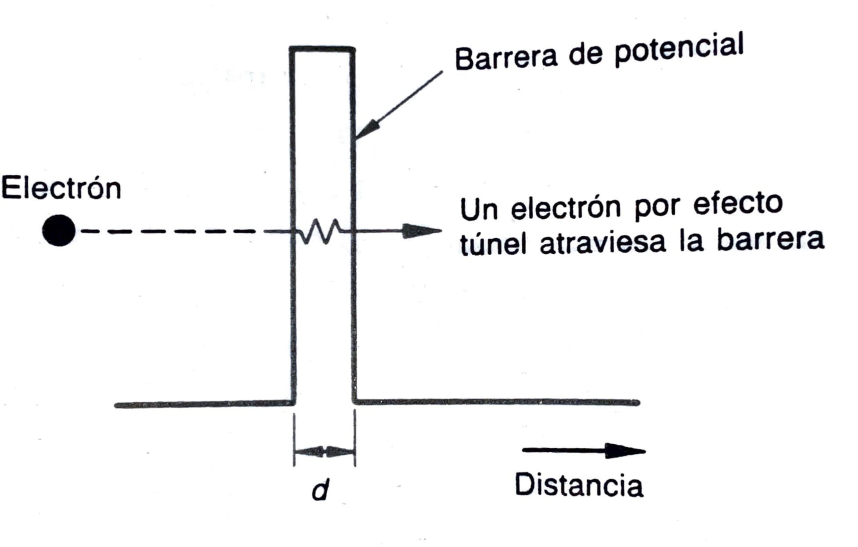
\includegraphics[width=0.9\textwidth]{Cuerpo/Ch_03/03_Temario_09.png}
    \end{subfigure}
    \begin{subfigure}{0.47\textwidth}
        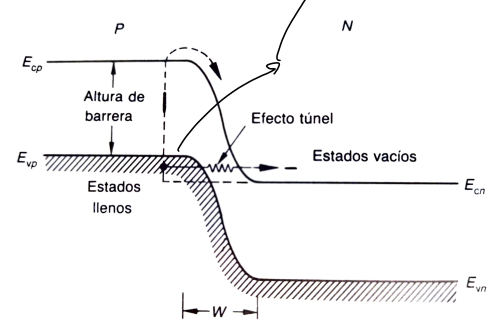
\includegraphics[width=\textwidth]{Cuerpo/Ch_03/03_Temario_08.png}
    \end{subfigure}
    \caption{rutpura zéner o por efecto túnel.}
\end{figure}

\subsubsection{Generación en la región de vaciamiento}


La generación en la región de vaciamiento aumenta negativamente la corriente de saturación inversa. En la deducción de la ecuación del diodo ideal consideramos que no existía RG en la zona de vaciamiento. Cuando $V<0$, predomina la generación, tal que estso portadores generados térmicamente contribuyen a la corriente en el circuito externo, produciendo una corriente adicional: 

\begin{equation}
    I_{\text{sal}} = I_{\text{RG}} + I_{\text{ideal}}
\end{equation}
donde 

\begin{equation}
    I_{\text{RG}} = - q A \int_{-x_p}^{x_n} G \D x
\end{equation}
siendo la tasa de generación: 

\begin{equation}
    G \approx \frac{n_i}{2\tau_0} \qquad \tau_0 = \frac{\tau_n+\tau_p}{2}
\end{equation}
Así: 

\begin{equation}
    I_{\text{RG}} = -q A \frac{n_i}{2\tau_0} W
\end{equation}
En el caso del silicio $I_{\text{RG}}$ es unas 50 veces más grande que $I_0$, mientras que en el germannio $I_0$ es unas 20 veces más grande que $I_{\text{RG}}$,

\subsubsection{Perforación}

La \textbf{perforación} se produce cuando la regió nde vaciamiento a través de la cual decae el potencial llega a un punto en el cual esta región en alguno de sus lados alcanza el contacto óhmico. Si el voltaje se incrementa más todavía, el contacto siente la penetración del campo eléctrico y suministra electrones hacia el diodo, el cual se cortocircuitda y las corrientes se limitan sólo por las resistencias del circuito externo. Se define el voltaje de perforación, $V_{\text{rp}}$, como la tensión que si se supera, el dispostivo entre en perforación. 

\subsection{Desviaciones en polarización directa}

Existen tres tipos de correciones o desviaciones en la curva IV cuando aplicamos polarización directa, que son:

\begin{itemize}
    \item Recombinación en la región de vaciamiento.
    \item Inyección de alto nivel.
    \item Efectos en la región masiva ($R_S\neq 0$).
\end{itemize}
Muchas veces la correción se ea través de un factor $n$ llamado \textbf{factor de idealidad} en la curva IV dada por el diodo ideal: 
parciales
\begin{equation}
    I = I_0 \parentesis{e^{qV_A/nkT}-1}
\end{equation}
\begin{figure}[h!] \centering
    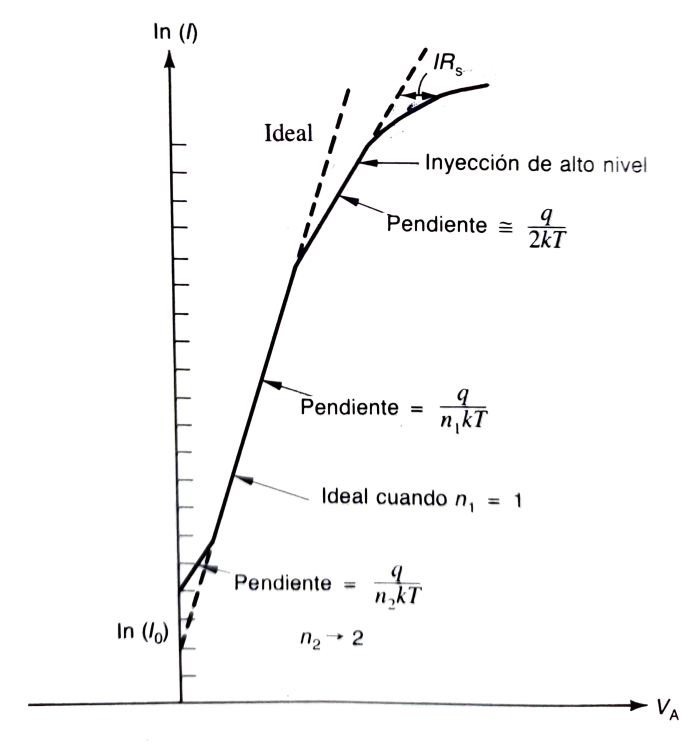
\includegraphics[width=0.5\linewidth]{Cuerpo/Ch_03/03_Temario_11.png}
    \caption{Corriente I respecto V en polarización directa.}
\end{figure}


\subsubsection{Recombinación en la región de vaciamiento}

Este proceso aumenta la corriente. Siguiendo el mismo proces que cuando estudiamos la generación en polarización inversa, cuando $V>0$ predomina la recombinación tal que: 

\begin{equation}
    I_{\text{RG}} = q A \frac{n_i}{2\tau_0} W \parentesis{e^{qV_A/n_2kT}-1}
\end{equation}
y así la intensidad total: 
\begin{equation}
    I = I_0 \parentesis{e^{qV_A/n_1kT}-1} +q A \frac{n_i}{2\tau_0} W \parentesis{e^{qV_A/n_2kT}-1}
\end{equation}

\subsubsection{Inyección de alto nivel}

La \textbf{inyección de alto nivel} se carga las ecuaciones del diodo ideal al no cumplir una de sus condiciones. Cuando estamos en a alto nivel de inyección las concentraciones minoritarias en exceso se acercan a la concentarción de portadores mayoritarios, y como la región masvia ha de mantener su neutraldiad de carga, la concentración de los portadores de mayoritarios también aumenta significativamente respecto a su valor del equilibrio. El resultado neto para $I$ es una dependencia 

\begin{equation}
    I = I_0 e^{qV_A/nkT}
\end{equation}
con $n>1$.

\subsubsection{Efectos en la región masiva}

Los \textbf{efectos en la región masiva} implican un estudio del diodo sin consdierar qeu el campo eléctrico en las regiones masivas es nulo, esto es, ahora hay caída de voltaje en los contactos óhmicos y zonas masivas. Para intensidades elevadas estso factores empeizan a ser importantes, siendo preciso aumentar la tensión aplicada para compesnar estos efectos y obtener el mismo valor de la intensidad. 

Estos efectos se representan por una reistencia $R_s$ denominada \textit{resistencia serie}. La corriente del diodo detendrá entonces el crecimiento expoencialmente y tenderá a saturarse, llegando a un comportamiento lineal típico de dispositivos óhmicos. Así, el voltaje ideal se convierte:

\begin{equation}
    \Vbi - V_A \longrightarrow \Vbi - V_A - \Delta V
\end{equation}

%%%%%%%%%%%%%%%%%%%%%%%%%%%%%%%%%%%%%%%%%%%%%%%%%%%%%%%%%%%%%%%%%%%%%%%
%%%%%%%%%%%%%%%%%%%%%%%%%%%%%%%%%%%%%%%%%%%%%%%%%%%%%%%%%%%%%%%%%%%%%%%
%%%%%%%%%%%%%%%%%%%%%%%%%%%%%%%%%%%%%%%%%%%%%%%%%%%%%%%%%%%%%%%%%%%%%%%
%%%%%%%%% CAPACIDADES DE VACIAMIENTO Y CIRCUITO EQUIVALENTE %%%%%%%%%%%
%%%%%%%%%%%%%%%%%%%%%%%%%%%%%%%%%%%%%%%%%%%%%%%%%%%%%%%%%%%%%%%%%%%%%%%
%%%%%%%%%%%%%%%%%%%%%%%%%%%%%%%%%%%%%%%%%%%%%%%%%%%%%%%%%%%%%%%%%%%%%%%
%%%%%%%%%%%%%%%%%%%%%%%%%%%%%%%%%%%%%%%%%%%%%%%%%%%%%%%%%%%%%%%%%%%%%%%


\section{Capacidades de vaciamiento y difusión}

Cuando nosotros aplicamos tensión en nuestro diodo, en la zona de vaciamiento aparece una carga $\rho$ no nula. Si nos damos cuenta, la disposición de la carga en el dispostivo se parece bastante a un condensador de placas planas paralelas (con la salvedad que las placas son planas):

\begin{figure}[h!] \centering
    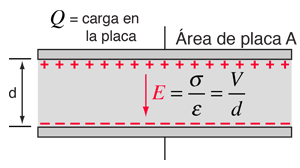
\includegraphics[width=0.45\linewidth]{Cuerpo/Ch_03/03_Temario_07.png}
    \caption{Capacitor de placas plano paralelas.}
\end{figure}
Y, de hecho, cuando modificamos el tamaño de la región de vaciamiento estamos modificando su carga total, y como sabemos, la capacidad de un dispositivo viene dada por: 

\begin{equation}
    C \equiv \abs{\derivadas{Q}{V}}
\end{equation}
Sin embargo no solo tenemos la carga total en la zona de vacimiento, el número de portadores minoritarios. Sin embargo, ¿Cómo es posible que los portadores minoritarios influyan en la capacidad si estos no aportan una carga neta? Aunque es cierto los portadores minoritarios no alteren la carga neta, sí contribuyen a la capacitancia porque son portadores móviles cuya densidad depende del voltaje. La capacitancia no depende de que haya un desbalance neto de carga, sino de cuánta carga móvil hay en función del voltaje aplicado. Así distinguimos dos tipos de capacitacias o capacidades: 

\begin{itemize}
    \item Capacidad de vaciamiento.
    \item Capacidad de difusión.
\end{itemize}
Consecuentemente un diodo no es solo modifica la intensidad total que puede circular a través de el, si no que también tiene una capacidad (con dos orígenes). Podremos expresar entonces la respuesta del diodo en un circuito a través de un circuito equivalente formado por una resistencia y dos capacitores. 

\subsection{Capacidad de vaciamiento}

Como sabemos la carga total vendrá dada por: 

\begin{equation}
    Q = q A x_n N_D = q A x_p N_A = q A \ccorchetes{\frac{K_S \epsilon_0}{2q} (\Vbi-V_A) \frac{N_AN_D}{N_D+N_A}}^{1/2}
\end{equation}
tal que la \textbf{capacidad de vaciamiento} es

\begin{equation}
    C_J = \abs{\derivadas{Q}{V_A}} = A \ccorchetes{\frac{2qK_S \epsilon_0}{\Vbi-V_A} \frac{N_AN_D}{N_D+N_A}}^{1/2} 
\end{equation}
que como podemos ver, usando que

\begin{equation}
    W = x_n + x_p = \ccorchetes{\frac{K_S \epsilon_0}{2q} (\Vbi-V_A) \frac{N_A+N_D}{N_DN_A}}^{1/2}
\end{equation}
tenemso que 

\begin{equation}
    C_J = \frac{AK_S\epsilon_0}{W} = \frac{A\epsilon}{W}
\end{equation}
es decir, igual que la que tendríamos en un capacitor de placas plano paralelas. 
\subsection{Capacidad de difusión}

En el diodo polarizado en directa la densidad de carga inyectada es bastnate grande, y puede dominar la capacidad. La carga del hueco inyectado en la región masiva N es: 

\begin{equation}
    Q_p = qA  \int_{x_n}^{\infty} (p_n-p_{n0} )\D x =  q A \int_{x_n}^{\infty} p_{n0} \parentesis{e^{qV/kT}-1} e^{-(x-x_n)/L_P} \D x 
\end{equation}
\begin{equation}
    Q_p = q A p_{n0} L_P  \parentesis{e^{qV/kT}-1}  
\end{equation}
de tal modo que la \textbf{capacidad de difusión}

\begin{equation}
    C_{\text{difusion}} = \abs{\derivadas{Q}{V}} =  \frac{q^2}{kT}A p_{n0} L_P  e^{qV/kT} = \frac{q}{kT} I \tau_p
\end{equation}

\subsection{Circuito equivalente}

Para estudiar el circuito equivalente de un diodo tendremos dos posibildiades, la \textbf{pequeña señal} esto es, cuando está en directa o en inversa exclusivamente pero se le superpone una señal alterna mucho más pequeña que la continua, o la \textbf{conmutación}, en el que el diodo pasa de estado inversa a continua. P

\subsubsection{Pequeña señal}

Primero hemos de evaluar la conductancia, que viene dada por:

\begin{equation}
    G = \derivadas{I}{V} = \frac{q}{kT} I(V)
\end{equation}
siendo esta coincidente con el invereso de la resistencia del diodo:

\begin{equation}
    G = \frac{1}{R} \approx \frac{I(\unit{mA})}{25.86} \Omega^{-1}
\end{equation}
Sin embargo el diodo también tiene capacidades no nulas, esto es, no se comporta igual en alterna que en continua.
Hemos supuesto que el diodo tenía únicamente comportamiento resistivo, sin embargo un diodo en señal alterna no se comporta de la misma forma que en continua. ¿Cómo? El circuito equivalente: 

\begin{figure}[h!] \centering
    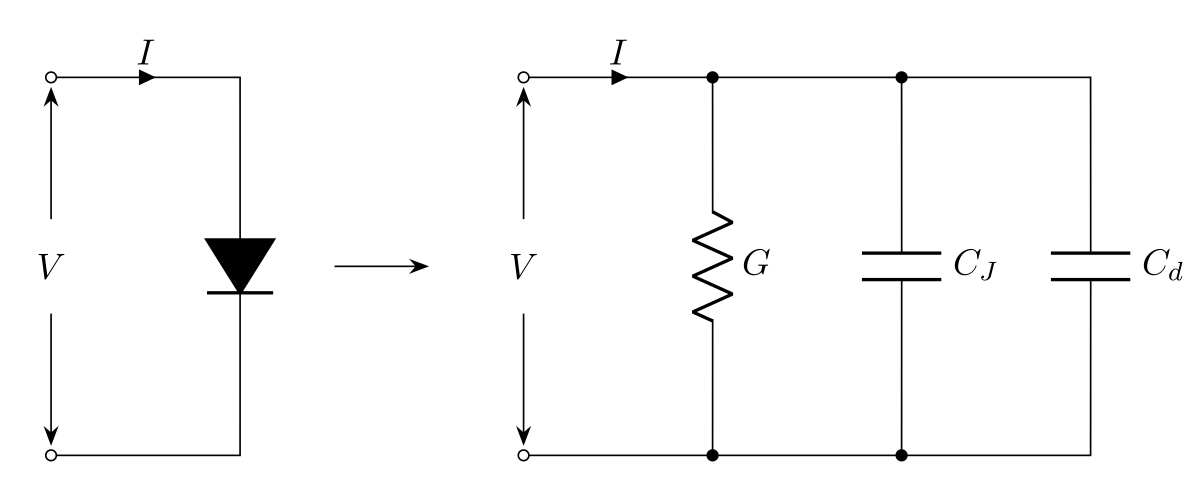
\includegraphics[width=0.6\linewidth]{Cuerpo/Ch_03/03_Temario_12}
\end{figure}
De lo qeu podemos sacar que la respuesta de la intensidad para un voltaje $v$  (ahora en minúscula porque es una señal alterna) en \textit{polarización directa}

\begin{equation}
    i = G v + C_{\text{difusion}} \derivadas{v}{t} 
\end{equation}
En el caso de \textit{polarización inversa}:
\begin{equation}
    i = G v + C_{\text{vaciamiento}} \derivadas{v}{t} 
\end{equation}

\subsubsection{Conmutación}

En general, las condiciones de la \textbf{polarización directa} en corriente alterna no es buena, ya que el flujo de corriente se debe a la inyección de carga minoritario, necesitando eliminar el exceso de carga minoritaria. La velocidad a la que se elimina depende de la recombinación o de la extracción por los contactos (diodos estrechos). En el caso de la \textbf{polarización inversa} como no se presenta ninguna inyección de carga minoritaria, la velocidad del dispositivo puede ser bastante alta. 

%%%%%%%%%%%%%%%%%%%%%%%%%%%%%%%%%%%%%%%%%%%%%%%%%%%%%%%%%%%%%%%%%%%%%%%
%%%%%%%%%%%%%%%%%%%%%%%%%%%%%%%%%%%%%%%%%%%%%%%%%%%%%%%%%%%%%%%%%%%%%%%
%%%%%%%%%%%%%%%%%%%%%%%%%%%%%%%%%%%%%%%%%%%%%%%%%%%%%%%%%%%%%%%%%%%%%%%
%%%%%%%%%%%%%%%%%%%%%%%%% HETEROUNIONES %%%%%%%%%%%%%%%%%%%%%%%%%%%%%%%
%%%%%%%%%%%%%%%%%%%%%%%%%%%%%%%%%%%%%%%%%%%%%%%%%%%%%%%%%%%%%%%%%%%%%%%
%%%%%%%%%%%%%%%%%%%%%%%%%%%%%%%%%%%%%%%%%%%%%%%%%%%%%%%%%%%%%%%%%%%%%%%
%%%%%%%%%%%%%%%%%%%%%%%%%%%%%%%%%%%%%%%%%%%%%%%%%%%%%%%%%%%%%%%%%%%%%%%


\section{Heterouniones}

Llmamamos \textbf{heterounión} a cualquier dispositivo PN que esté formado por dos tipos didferenets de material, por ejemplo GaAs en la zona N y GaAl en la zona P. Para poder formar una heterounión necesitamos que los dos materiales tengan una constante de red similar, lo cual es complicado. 




